\graphicspath{{figures/results/}}
\chapter{Results}
The results presented are both training and testing results from the two solutions. Both the image classification and the multi-class object detection are trained and tested on the 60 seconds video with three zebrafish.

The solutions are trained on annotated data of 411 different occlusions in total and a similar amount annotated occurrences of \textit{no occlusions}.

\section{Image Classification}
The image classification solution is trained for 15 epochs, the results are shown in \autoref{fig:img_class-15ep}
\begin{figure}[H]
	\centering
	\begin{subfigure}{0.48\textwidth}
		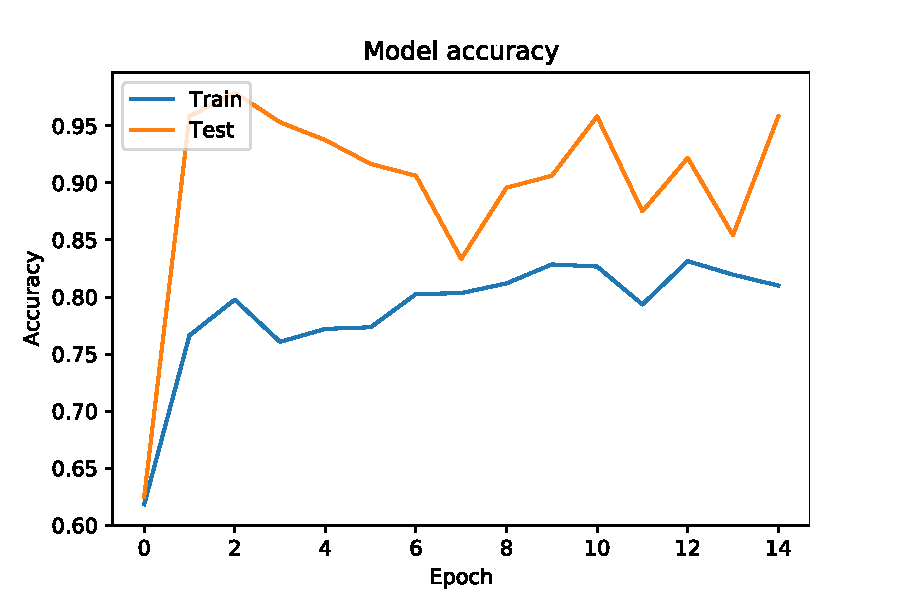
\includegraphics[width=\textwidth]{model_acc_15epoch}
		\caption{The image classification accuracy for both training and testing}
		\label{fig:img_acc-15}
	\end{subfigure}
	\begin{subfigure}{0.48\textwidth}
		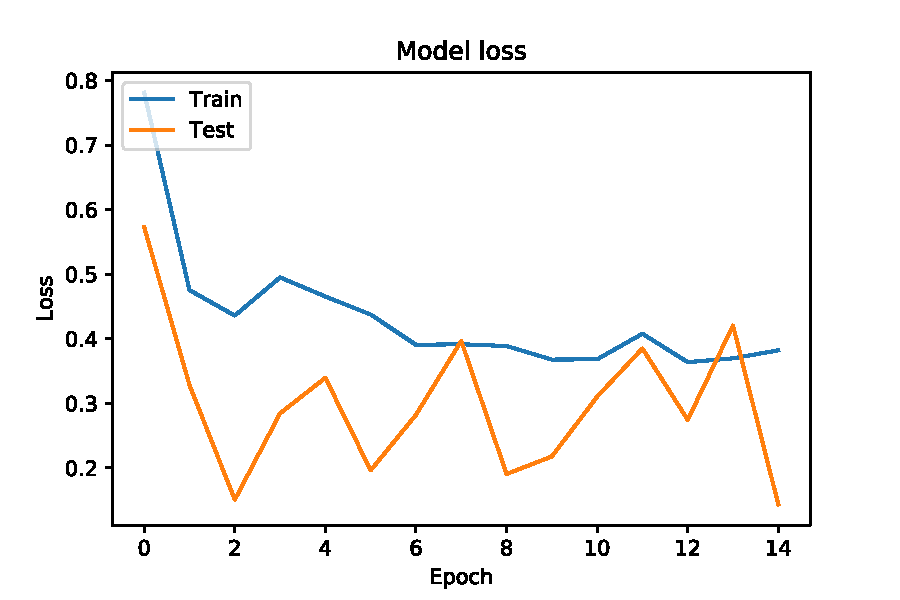
\includegraphics[width=\textwidth]{model_loss_15epoch}
		\caption{The image classification loss for both training and testing}
		\label{fig:img_loss-15}
	\end{subfigure}
\caption{Model accuracy and loss when trained for 15 epochs}
\label{fig:img_class-15ep}
\end{figure}

As shown in \autoref{fig:img_class-15ep} the training accuracy is lower than the testing accuracy, however, the training graph is in both functions more stable and seems closer to converging than the testing graph. Meanwhile, the training loss is  higher than the test loss as well.

In general, the model is still unstable and needs more training for converging.

\autoref{tab:img_class_15ep} also shows that the test results are better than the training.
\begin{table}[H]
	\centering
	\caption{End results achieved with 15 epochs.}
	\begin{tabular}{|l|l|}
		\hline
		Training Loss                	& 0.4841 			\\\rowcolor{lightGrey}\hline
		Training Accuracy       	    & 0.7738 			\\ \hline
		Testing Loss     				& 0.2487 			\\\rowcolor{lightGrey}\hline
		Testing Accuracy 				& 0.9318			\\ \hline
	\end{tabular}
\label{tab:img_class_15ep}
\end{table}

The image detection model is also trained for 100 epochs, the results of this is shown in \autoref{fig:img_class-100ep} and \autoref{tab:img_class_100ep}.
\begin{figure}[H]
	\centering
	\begin{subfigure}{0.48\textwidth}
		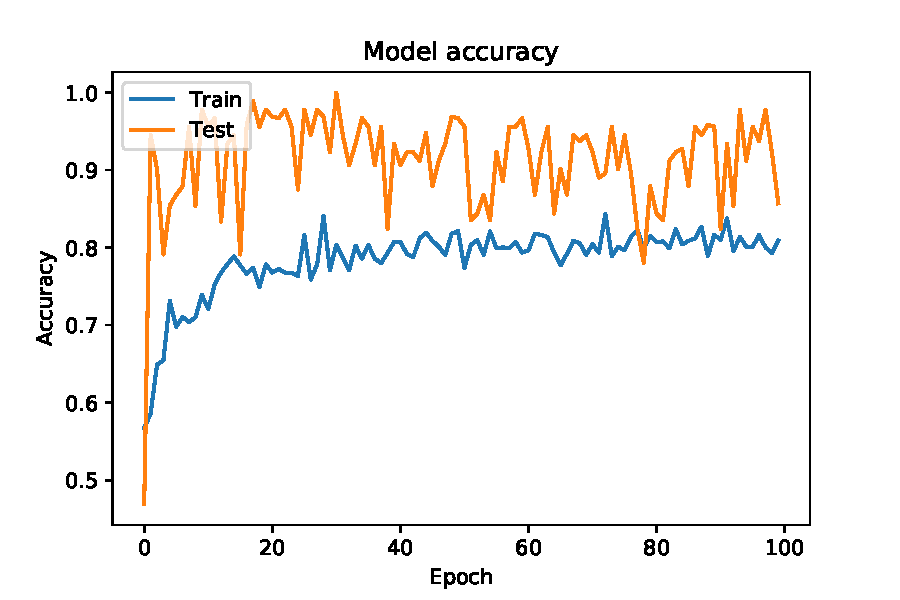
\includegraphics[width=\textwidth]{model_acc_100epoch}
		\caption{The image classification accuracy for both training and testing}
		\label{fig:img_acc-100}
	\end{subfigure}
	\begin{subfigure}{0.48\textwidth}
		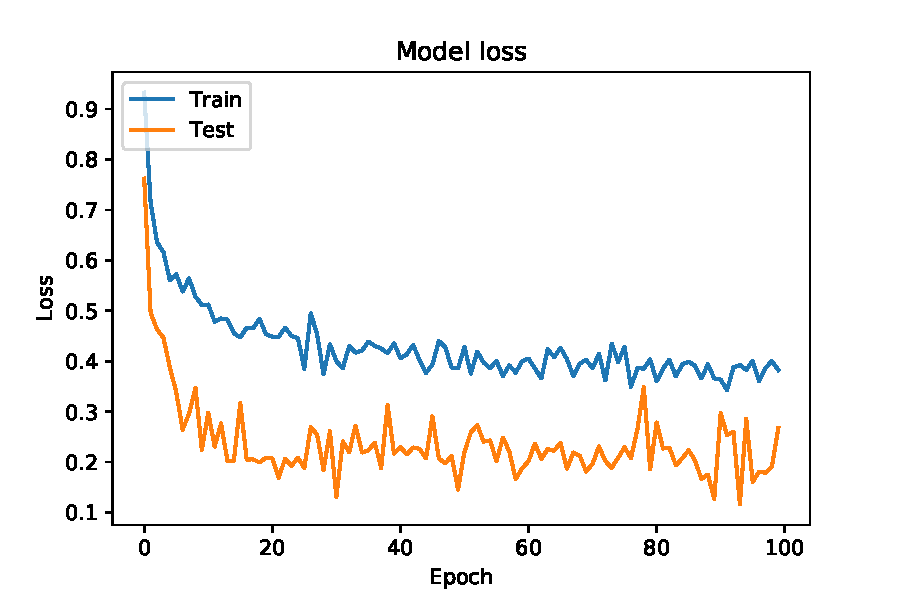
\includegraphics[width=\textwidth]{model_loss_100epoch}
		\caption{The image classification loss for both training and testing}
		\label{fig:img_loss-100}
	\end{subfigure}
\caption{Model accuracy and loss when trained for 100 epochs}
\label{fig:img_class-100ep}
\end{figure}
There is still a high amount of instability, but in general the test results are better than the training. It has tendencies towards converging, but it is uncertain due to the instability.

\begin{table}[H]
	\centering
	\caption{End results achieved with 100 epochs.}
	\begin{tabular}{|l|r|}
		\hline
		Training Loss            		& 0.3831	\\ \rowcolor{lightGrey}\hline
		Training Accuracy        	    & 0.8075 	\\ \hline
		Testing Loss     				& 0.2680	\\ \rowcolor{lightGrey}\hline
		Testing Accuracy 				& 0.8571	\\ \hline
	\end{tabular}
	\label{tab:img_class_100ep}
\end{table}

\section{Object Detection}
The Faster \gls{rcnn} object detection model is trained with a split of $85\%$ for training and $15\%$ for testing.

\subsection{Training}
Training is done at 42 and 152 epochs, as these points had an automatic stop. When training, the best performing weights are saved.

\subsubsection{42 Epochs}
After the object detection model has been trained for 42 epochs, the training accuracy is as shown in the following figures:
\begin{figure}[H]
	\centering
	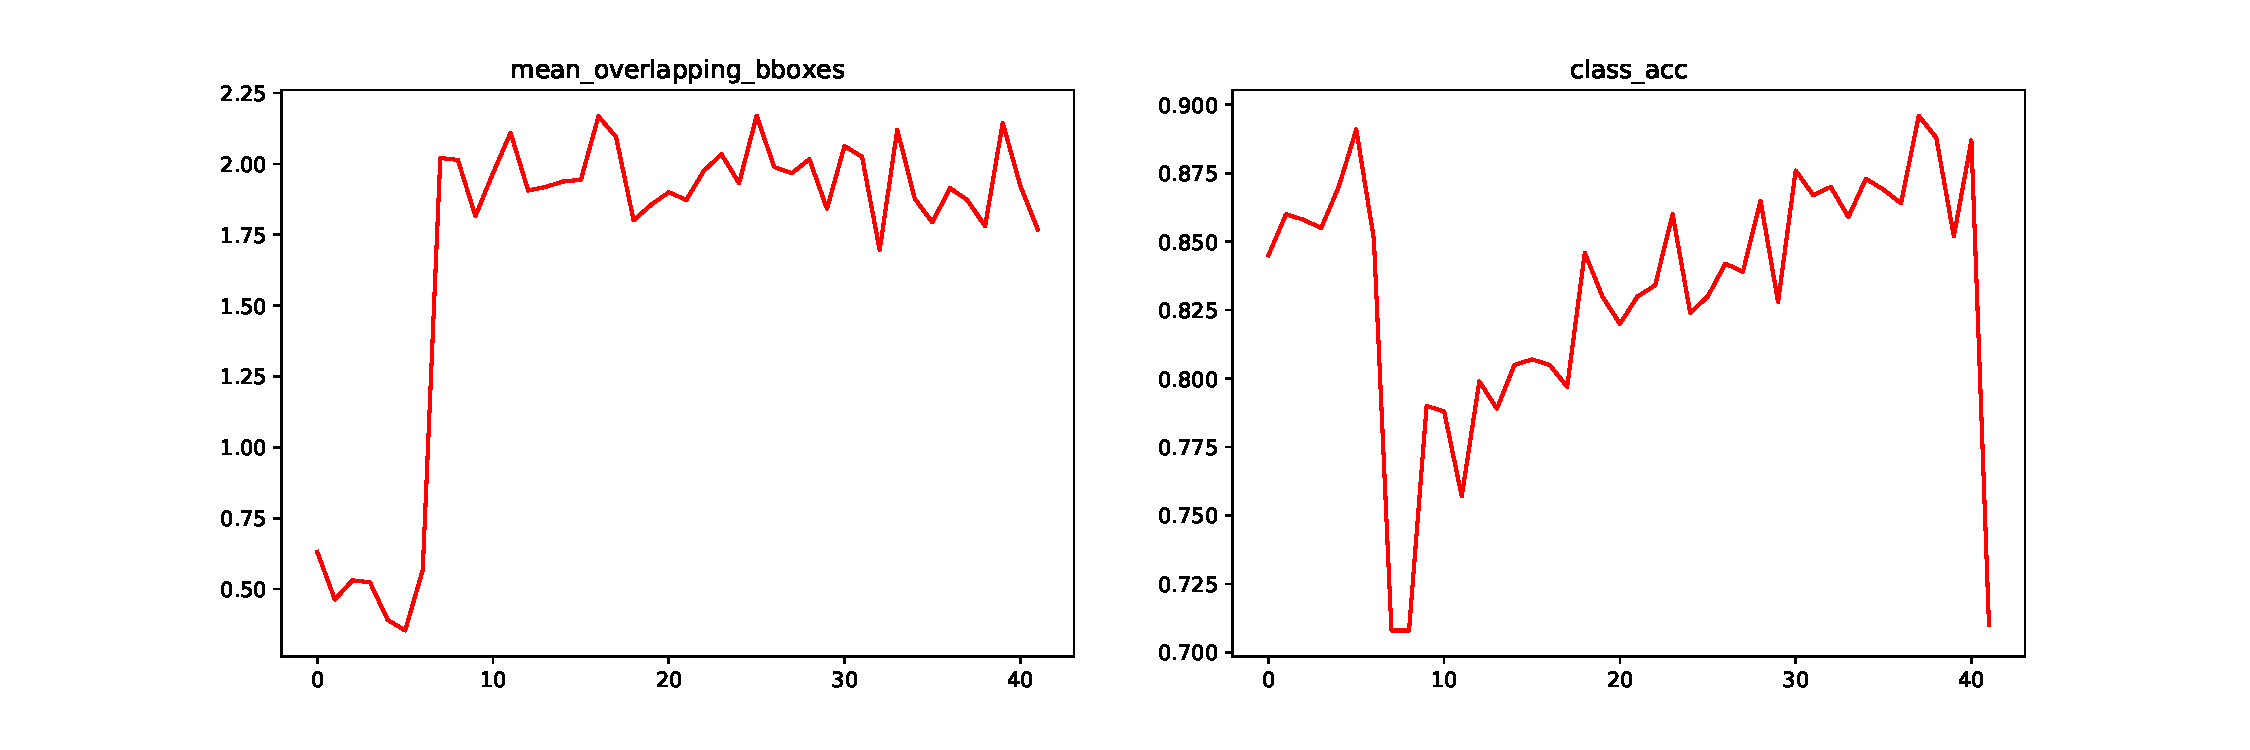
\includegraphics[width=\textwidth]{acc-42}
	\caption{Mean of overlapping bounding boxes of ground truth and classification accuracy}
	\label{fig:acc-42}
\end{figure}
\autoref{fig:acc-42} shows the mean overlapping bounding boxes of the ground truth bounding box, and the classification accuracy of the \gls{rcnn} classifier.

\begin{figure}[H]
	\centering
	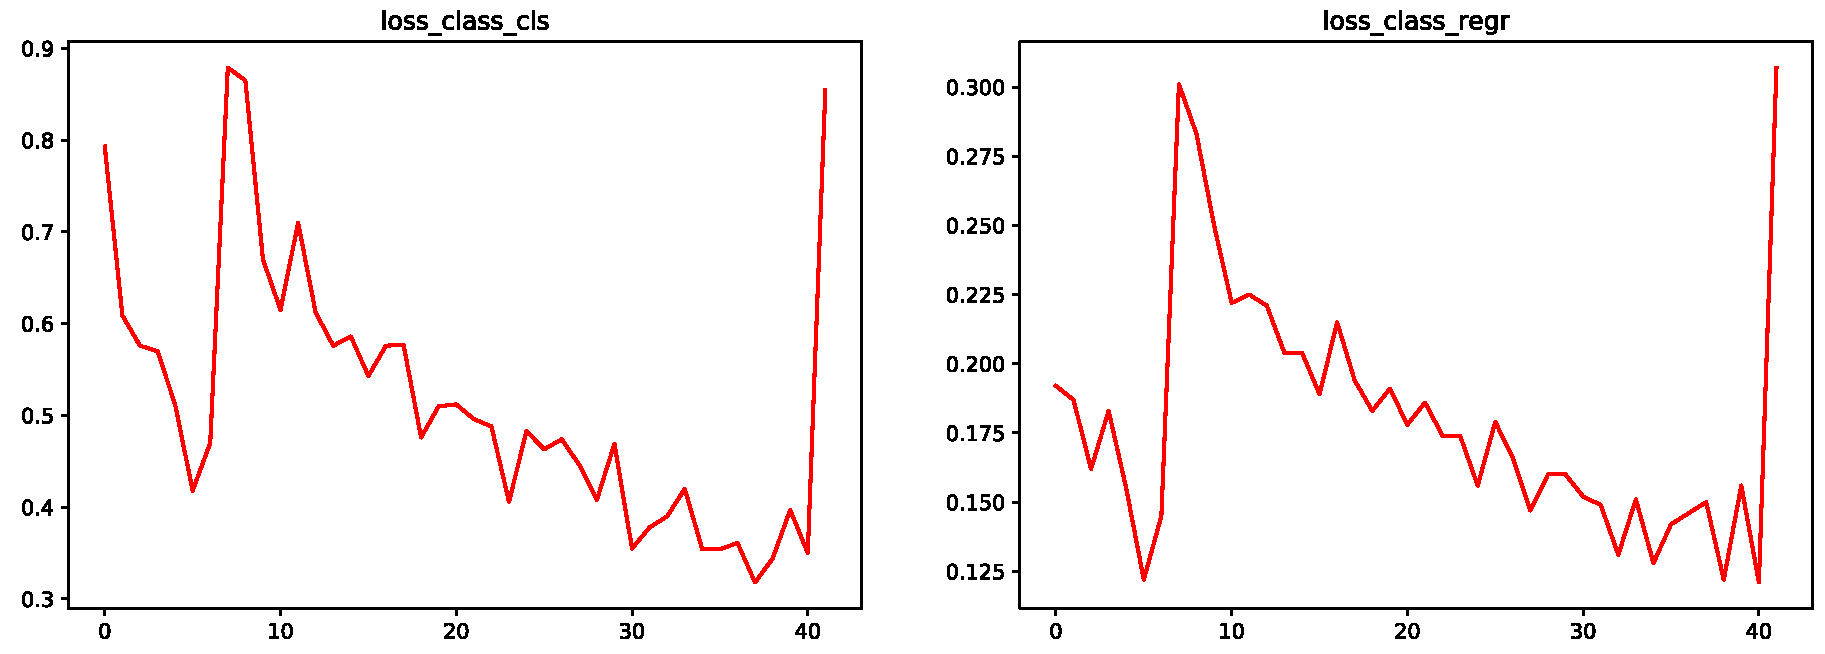
\includegraphics[width=\textwidth]{loss_class-42}
	\caption{Loss in classification and general bounding box regression}
	\label{fig:loss_class-42}
\end{figure}
\autoref{fig:loss_class-42} shows the loss in the \gls{rcnn} classifier and bounding box regression.

\begin{figure}[H]
	\centering
	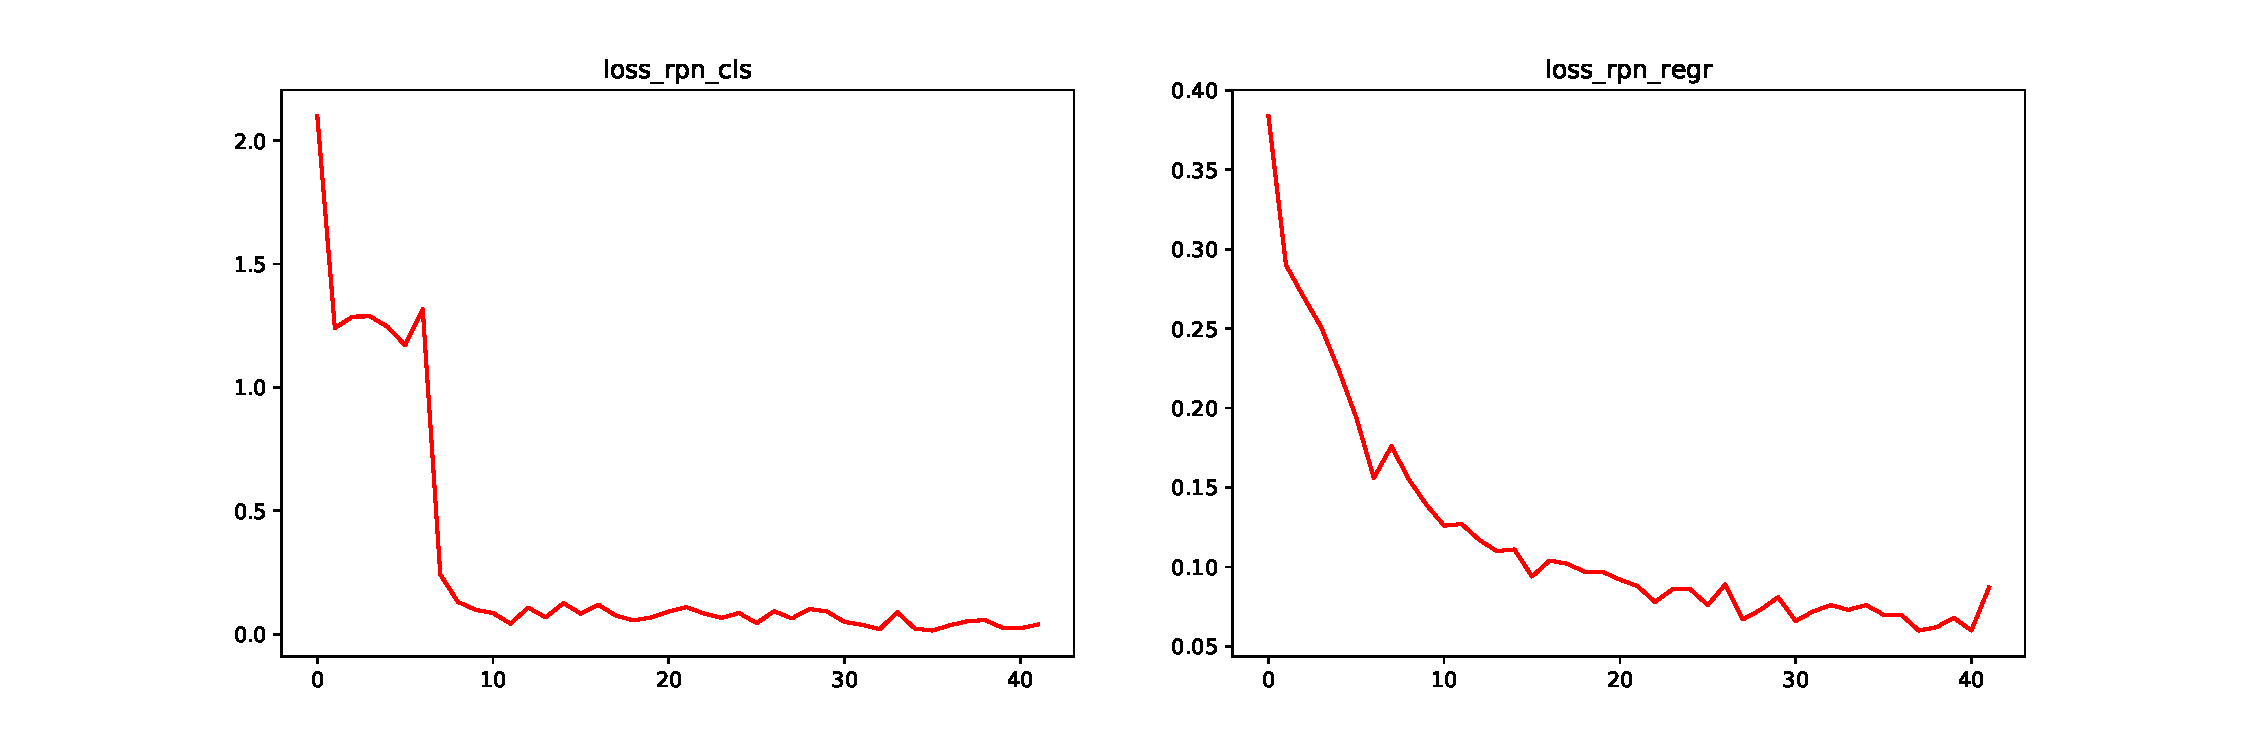
\includegraphics[width=\textwidth]{loss_rpn-42}
	\caption{Loss in the \gls{rpn} classification and general bounding box regression}
	\label{fig:loss_rpn-42}
\end{figure}
\autoref{fig:loss_rpn-42} shows the loss in the \gls{rpn} classifier and bounding box regression.

\begin{figure}[H]
	\centering
	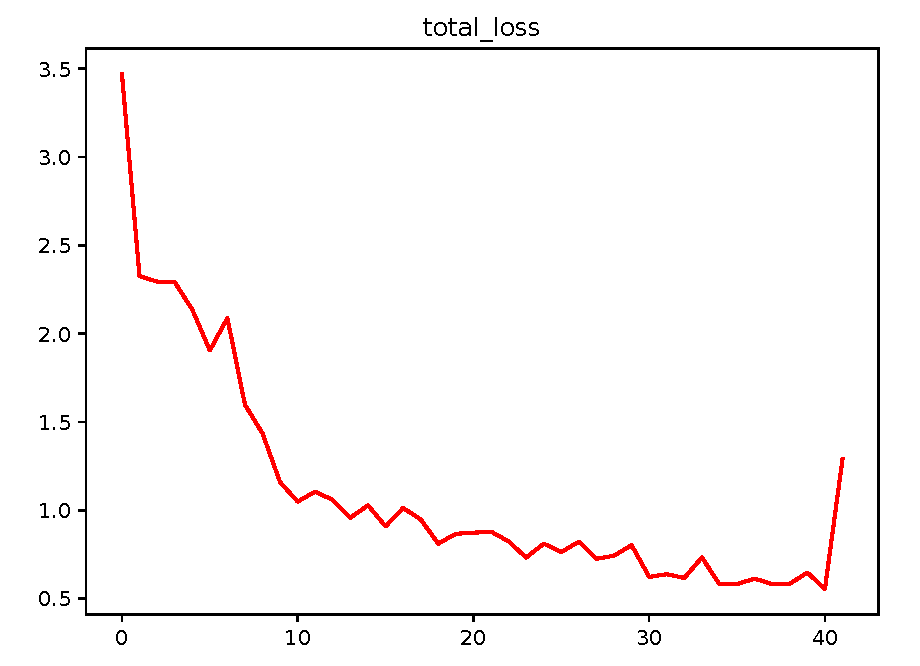
\includegraphics[width=0.7\textwidth]{total_loss-42}
	\caption{Total loss of the entire model}
	\label{fig:total_loss-42}
\end{figure}
\autoref{fig:total_loss-42} shows the total loss of the model during training. The \gls{rcnn} classification and regression steps show signs of instability, which is seen in the loss and the accuracy of both overlapping bounding boxes and the classification accuracy.

When testing with these results, the test was stopped due to poor performance.

\subsubsection{152 Epochs}
After the object detection model has been trained for 152 epochs, the training accuracy is as shown in the following figures:
\begin{figure}[H]
	\centering
	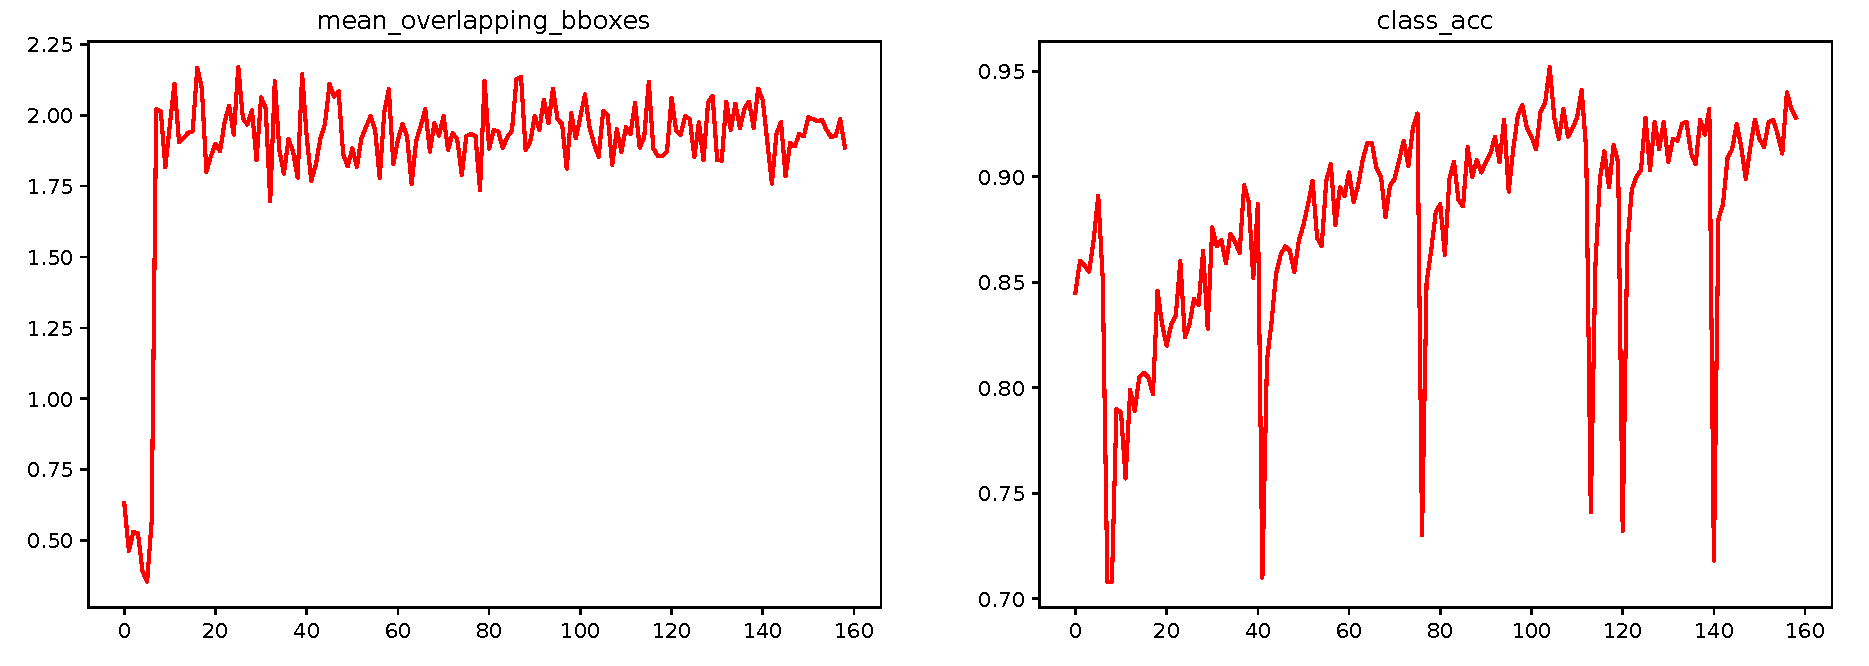
\includegraphics[width=\textwidth]{acc-152}
	\caption{Mean of overlapping bounding boxes of ground truth and classification accuracy}
	\label{fig:acc-152}
\end{figure}
\autoref{fig:acc-152} shows the mean overlapping bounding boxes of the ground truth bounding box, and the classification accuracy of the \gls{rcnn} classifier.

\begin{figure}[H]
	\centering
	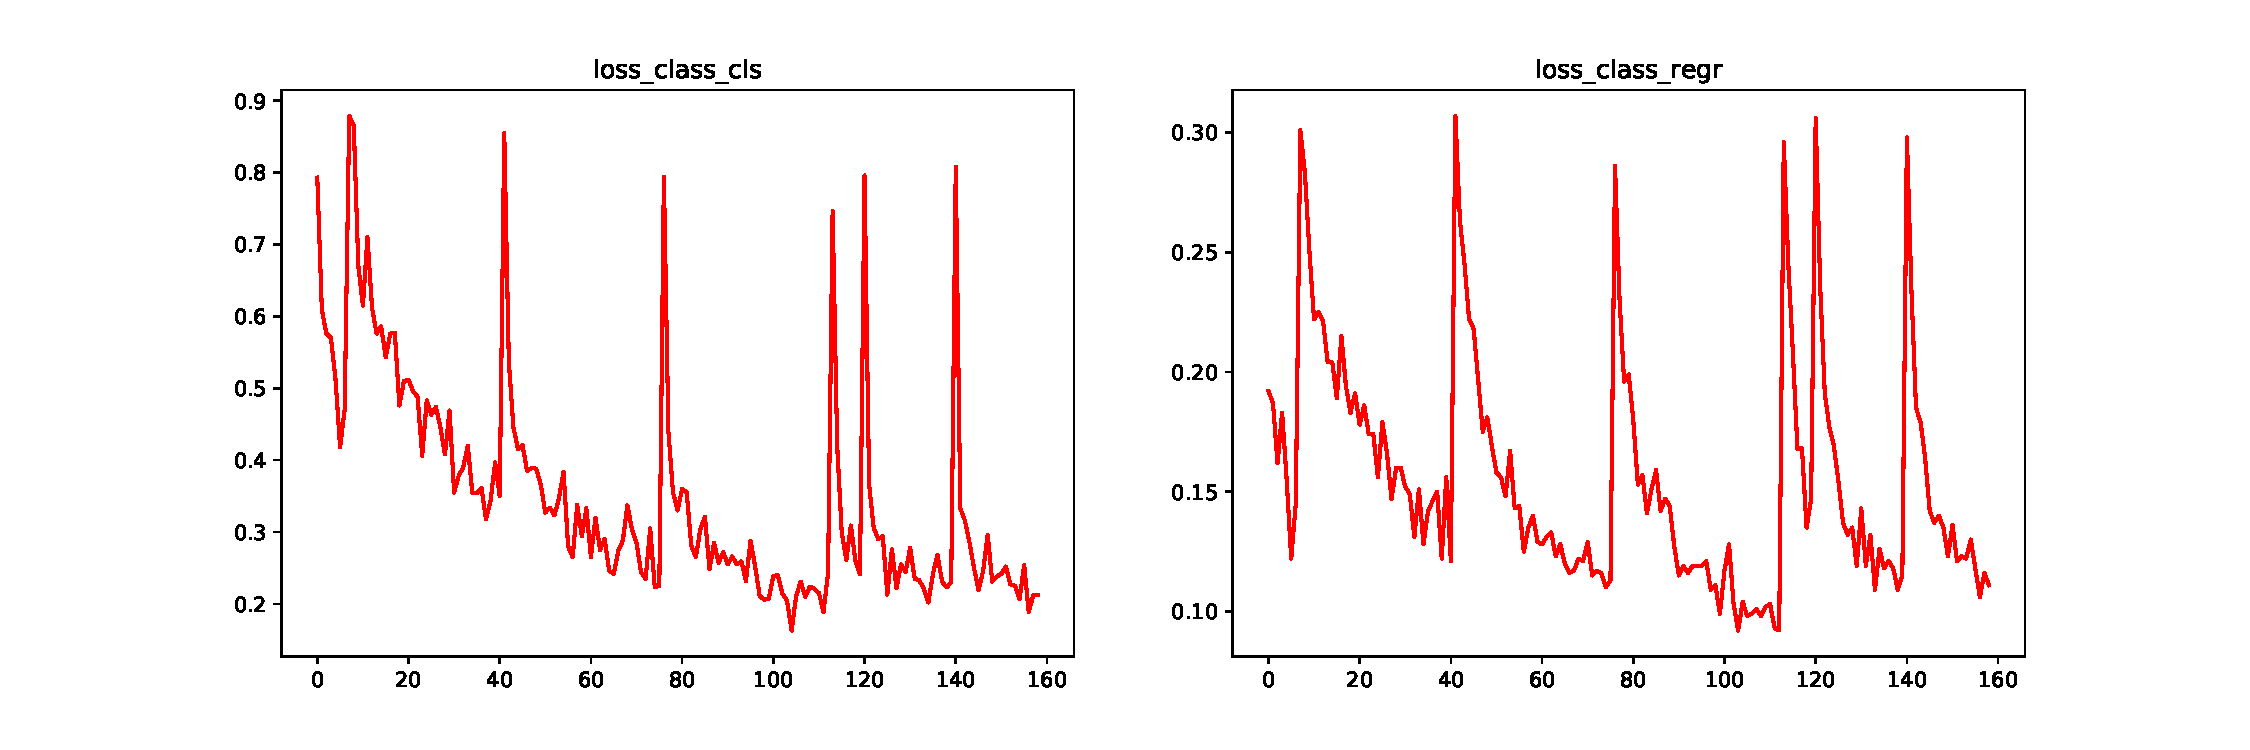
\includegraphics[width=\textwidth]{loss_class-152}
	\caption{Loss in classification and general bounding box regression}
	\label{fig:loss_class-152}
\end{figure}
\autoref{fig:loss_class-152} shows the loss in the \gls{rcnn} classifier and bounding box regression.

\begin{figure}[H]
	\centering
	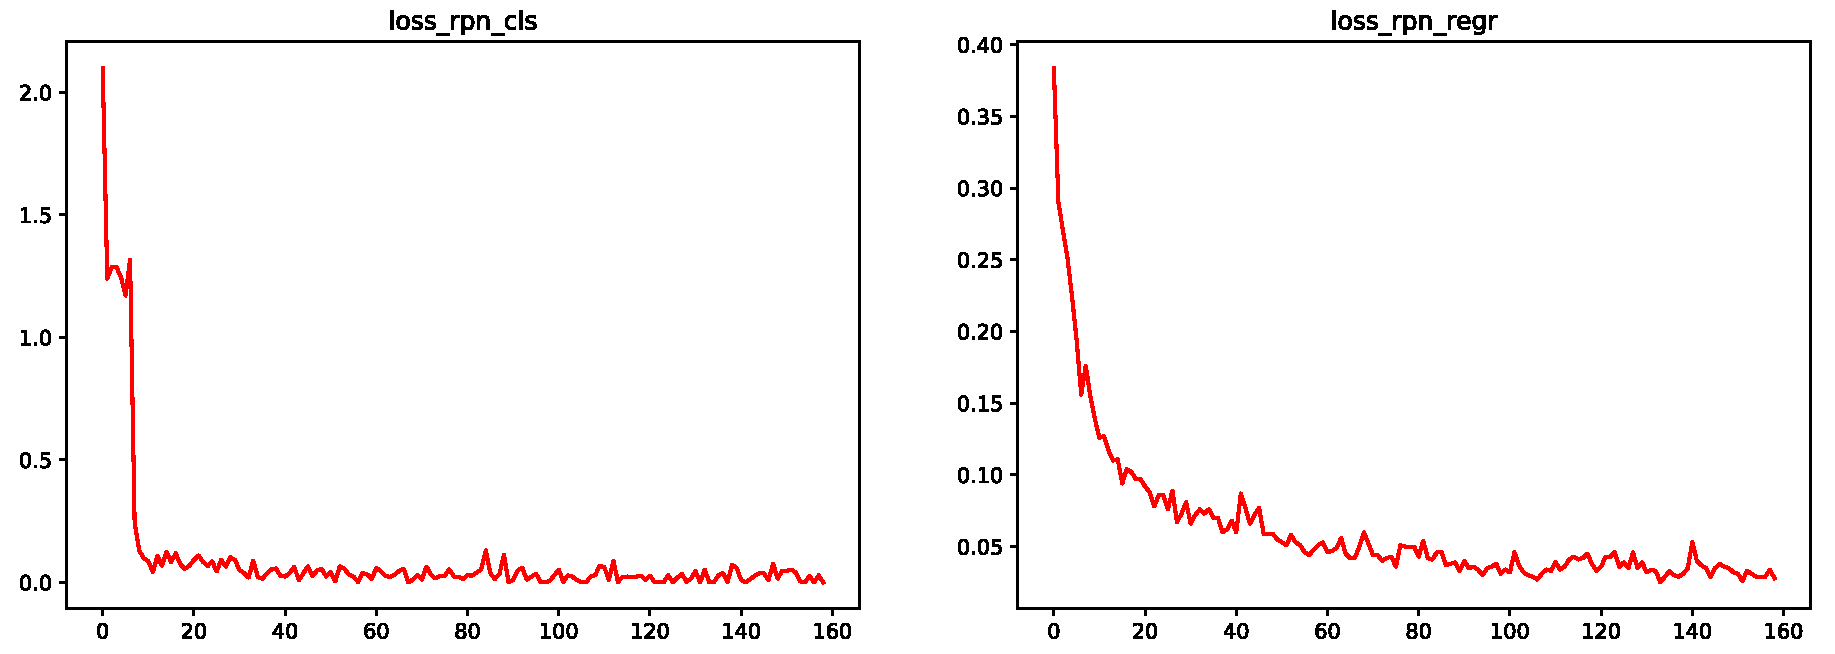
\includegraphics[width=\textwidth]{loss_rpn-152}
	\caption{Loss in the \gls{rpn} classification and general bounding box regression}
	\label{fig:loss_rpn-152}
\end{figure}
\autoref{fig:loss_rpn-152} shows the loss in the \gls{rpn} classifier and bounding box regression.

\begin{figure}[H]
	\centering
	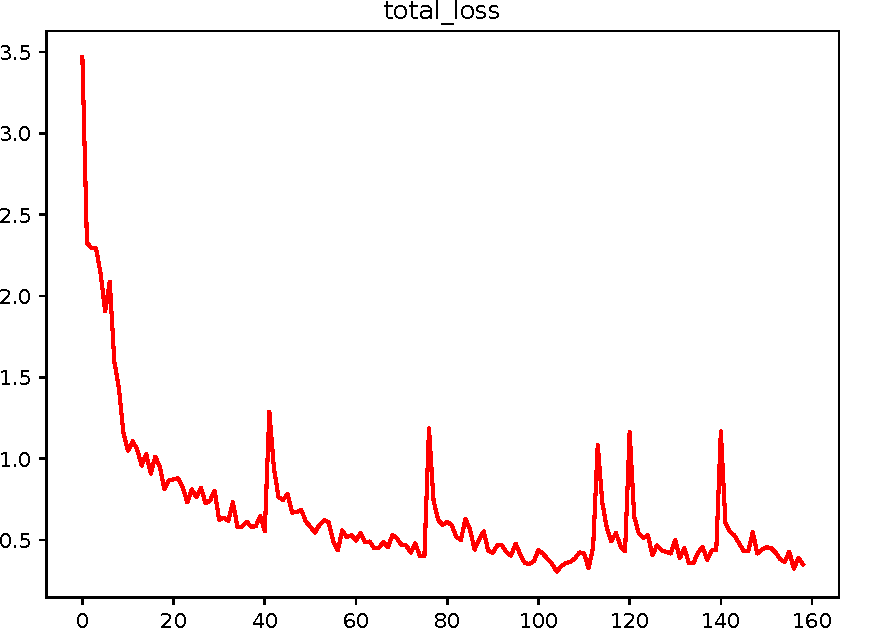
\includegraphics[width=0.7\textwidth]{total_loss-152}
	\caption{Total loss of the entire model}
	\label{fig:total_loss-152}
\end{figure}
\autoref{fig:total_loss-152} shows the total loss of the model during training. There are still signs of instability and again especially in the \gls{rcnn} classification and regression. However, there are signs towards the model converging.

\subsection{Testing}
The training and testing split is $85\%$ for training and $15\%$ for testing. With this split the solution reaches a \gls{map} of $66.8\%$.

\autoref{fig:T-det}, \ref{fig:not-det}, and \ref{fig:no-occl-det} show plots of predictions of three random testing frames, with predictions and bounding box regressions. The predictions and the accuracy is written in the image caption. Only detections with a confidence above $70\%$ are accepted.\\

\autoref{tab:class-pred} shows that the average precision is very different between classes, ranging from $34.4\%$ to $ 100\% $.
\begin{table}[H]
	\centering
	\caption{Average precisions of the different occlusion types}
	\label{tab:class-pred}
	\begin{tabular}{lr}
		\textbf{Occlusion Type} & \textbf{Average Precision} \\\rowcolor{lightGrey}\hline
		T Shape                 & $ 74.6\% $                     \\
		V Shape                 & $ 53.9\% $                    \\\rowcolor{lightGrey}
		On Top                  & $ 100\% $                      \\
		Cross                   & $ 78.2\% $                     \\\rowcolor{lightGrey}
		Elongation              & $ 91.9\% $                     \\
		Other                   & $ 37.6\% $                     \\\rowcolor{lightGrey}
		No Occlusion            & $ 34.6\% $                    
	\end{tabular}
\end{table}



\autoref{fig:T-det} shows two zebrafish creating a T-shape occlusion, which is detected with a confidence of $91.37\%$ and single zebrafish detected as no occlusion with a confidence of $99.48\%$.
\begin{figure}[H]
	\centering
	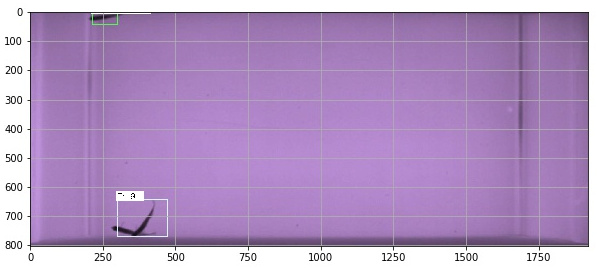
\includegraphics[width=\textwidth]{prediction-frame596}
	\caption{Detection of the T-shape is with a confidence of $91.37\%$ and of no occlusion with $99.48\%$}
	\label{fig:T-det}
\end{figure}

\autoref{fig:not-det} shows a crossing occlusion which is not being detected and a single zebrafish detected as no occlusion with a confidence of $99.43\%$.
\begin{figure}[H]
	\centering
	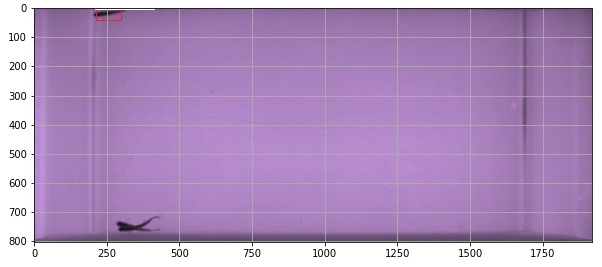
\includegraphics[width=\textwidth]{prediction-frame601}
	\caption{Only detection of no occlusion with confidence of $99.43\%$}
	\label{fig:not-det}
\end{figure}

\autoref{fig:no-occl-det} shows three zebrafish with no occlusions occurring in the image, but only two of them are detected as no occlusions, with confidences of $99.48\%$ and $98.73\%$. The last zebrafish does not have a detection confidence higher than $70\%$ and is therefore ignored.
\begin{figure}[H]
	\centering
	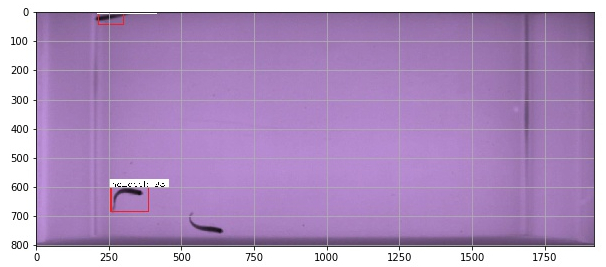
\includegraphics[width=\textwidth]{prediction-frame1092}
	\caption{Two detections of no occlusions with confidence of $99.48\%$ and $98.73\%$}
	\label{fig:no-occl-det}
\end{figure}